\subsection{Divider}


The algorithm implemented in the original version of the processor is one of the simplest but the
slowest available.

Several other algorithms can compute the division faster but all of them present disadvantages
that must be taken into account according to the target application.

Algorithms like repeated multiplication or reciprocation are fast but require a significant amount
of area, similarly an array divider would have been very fast only If we had control on the
place\&routing process in order to create a regular structure. In the end we decided to implement
a simple radix-4 division algorithm for simplicity of implementation and of the circuit itself.

Using an higher radix could have improved performance but the size of the lookup table required
by the algorithm would have increased again the area consumption.

The divider consist in a state machine (its diagram is shown in figure~\ref{fig:div_state_dia}) which checks if the inputs will
generate an overflow and performs a preliminary shift to put the divisor in the appropriate range
to be computed correctly.


\begin{figure}[H]
\centering
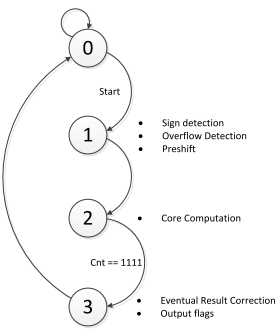
\includegraphics[width=0.85\textwidth,height=0.4\textheight,keepaspectratio]{DivisorStateMachine.png}
\caption{Divider State Diagram.}
\label{fig:div_state_dia}
\end{figure}

After that, the real computation begins and lasts 16 clock cycles. The block diagram of the divider
while it's in this state is shown in figure~\ref{fig:div_block_dia}.

\begin{figure}[H]
\centering
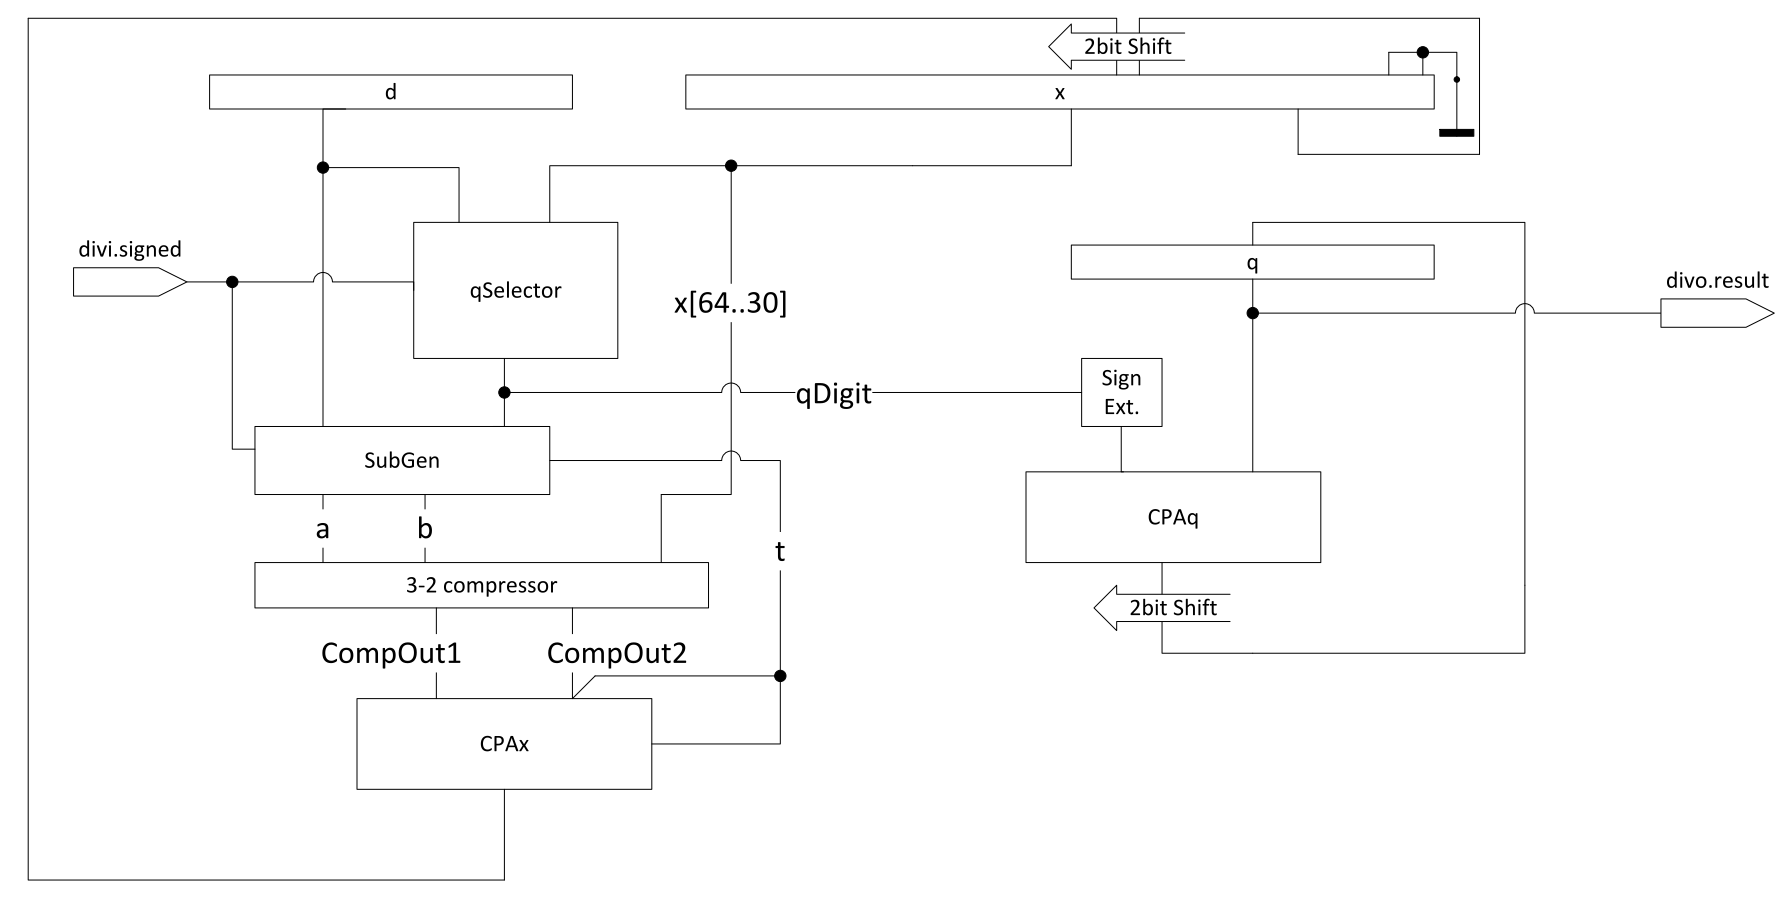
\includegraphics[width=0.85\textwidth,height=0.4\textheight,keepaspectratio]{DivisorDiagram.png}
\caption{Divider Block Diagram (during Core Computation, State = 1).}
\label{fig:div_block_dia}
\end{figure}

The algorithm is very similar to the original radix-2 version but in this case the partial reminder (x)
is shifted by 2 bits every cycle and the circuit has to guess the quotient digit from the range [-3,3].
``qSelector'' is the lookup table which performs the quotient digit guessing and it's based on the p-
d plot of the radix-4 SRT division shown in figure~\ref{fig:div_pd_plot}. In case of unsigned division only the right half of
the p-d plot is being used.

The quotient digits are in a radix-4 redundant format so a conversion to binary format is needed.
The conversion is performed gradually every cycle by the 32-bit adder ``CPAq'' which shift and sum
each generated digit with the already calculated quotient.

One could think that it would be better keep the quotient in a radix-4 redundant format and avoid
the addition in order not to slow down the execution every cycle so that the clock frequency could
be higher, but also the original divider executes a 32-bit addition every cycle so from this point of
view our divider is not worse than the original one, moreover a conversion from radix-4 redundant
format to binary is quite complicated, doing this it consists in a simple addition.

The same concept has been used also for the computation of the partial reminder.

An addition/subtraction in Carry-Save format would have been much faster and also easier, but
the selection of the quotient digit would have required the analysis of the most significant bits of
both the sum and the carry making the lookup table several orders of magnitude bigger.
In our divider ``SubGen'' generates the multiple of d to sum with the current partial reminder in a
carry save format, all this operands are been compressed by a 3-2 compressor (1 full adder of
delay) and finally the new partial reminder is calculated with a 35-bit adder, ``CPAx''

\begin{figure}[H]
\centering
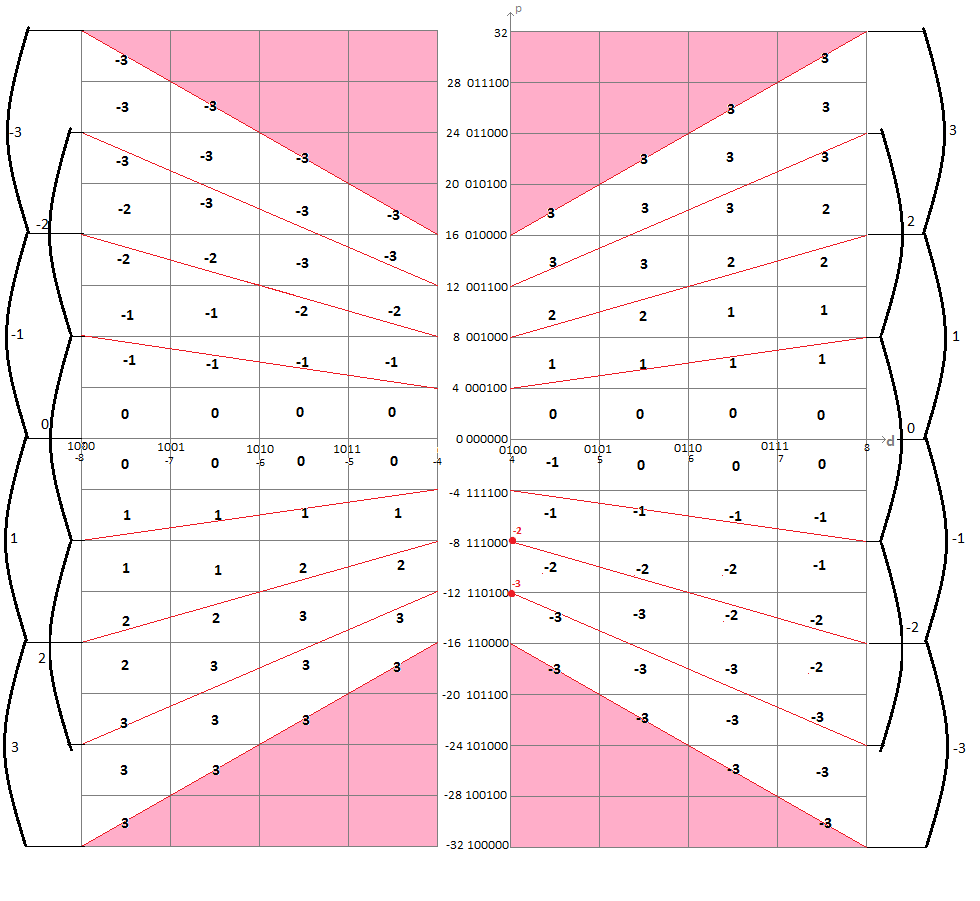
\includegraphics[width=0.85\textwidth,height=0.85\textheight,keepaspectratio]{radix4pd.png}
\caption{Radix-4 P-D Plot (Red Dots are Exceptions).}
\label{fig:div_pd_plot}
\end{figure}

Other solutions have been analyzed, such as having a lookup table only for unsigned division, half
of the size of the final version, and handle the sign separately but the synthesis has shown that the
resources utilization would have not changed significantly while one more cycle would have been needed.
Hence, we decided to keep the current divider.

At last, in order to check the compatibility of the radix-4 divider with the original one we
performed a simulation of the two versions with the same output, the only difference is in the
case of overflows where the flag is set up correctly but the result is different or in some cases
undefined, but since there is an overflow the result has no meaning so this is acceptable.

\begin{figure}[H]
\centering
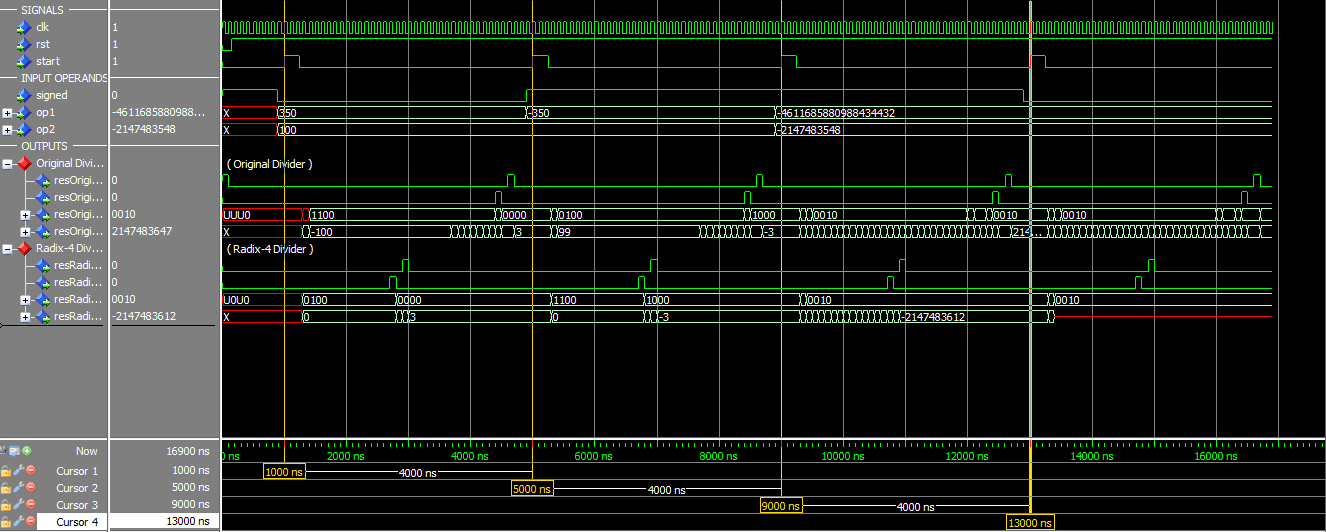
\includegraphics[width=1\textwidth,height=0.6\textheight,keepaspectratio]{myDivisionvsOriginal.png}
\caption{Signal Dump Of Radix-4 Divider Vs. Original Divider.}
\label{fig:div32_wave}
\end{figure}
